\documentclass[12pt]{article}
\usepackage[utf8]{inputenc}
\usepackage{graphicx}
\usepackage{geometry}
\usepackage{float}
\usepackage{amsmath}
\usepackage{caption}
\usepackage{subcaption}
\usepackage{hyperref}
\geometry{margin=1in}

\title{Emotion Detection in Persian Text using Machine Learning}
\author{Student Name \\ Shahid Beheshti University \\ Machine Learning Fundamentals – 3rd Assignment}
\date{June 2024}

\begin{document}

\maketitle

\begin{abstract}
This report presents a machine learning approach for detecting emotions in Persian text, categorized into five classes: happiness, sadness, anger, fear, and others. The methodology encompasses text preprocessing, feature engineering using TF-IDF, training with classical models such as logistic regression, and evaluating the results using precision, recall, and F1-score. The pipeline demonstrates the challenges and insights in multilingual NLP, especially on imbalanced data.
\end{abstract}

\section{Introduction}
Text-based emotion recognition is a crucial component in natural language understanding, with applications in sentiment analysis, mental health, and human-computer interaction. This report investigates a classical machine learning approach for detecting emotions in Persian texts. The dataset includes labeled samples with single-label classification into five emotional states.

\section{Data Preprocessing}
\subsection{Loading and Normalization}
The dataset was first loaded and Persian text normalization was applied to standardize characters and remove diacritics.

\subsection{Cleaning}
The following cleaning steps were applied:
\begin{itemize}
    \item Removal of punctuation, numbers, and special characters.
    \item Tokenization into words.
    \item Removal of Persian stopwords.
\end{itemize}

\subsection{Feature Engineering}
Texts were vectorized using TF-IDF, and labels were encoded using \texttt{LabelEncoder}.

\section{Exploratory Data Analysis (EDA)}
The first step in EDA involved examining class distributions and word frequencies. As seen in Figure \ref{fig:classdist}, the dataset is imbalanced, with most samples belonging to HAPPY and OTHER.

\begin{figure}[H]
    \centering
    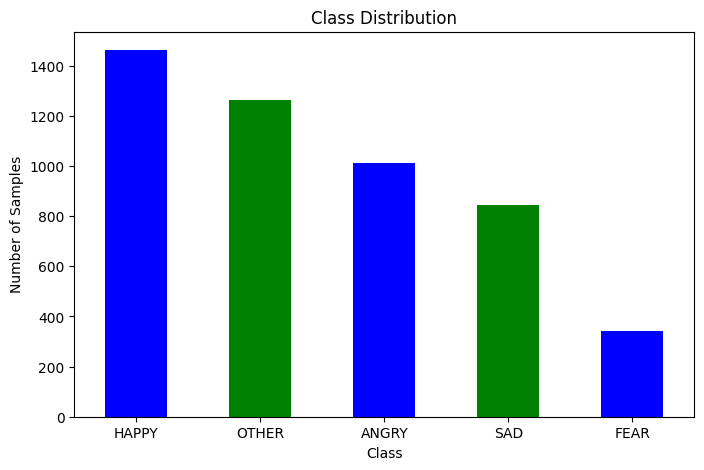
\includegraphics[width=0.7\textwidth]{output2.png}
    \caption{Class Distribution}
    \label{fig:classdist}
\end{figure}

The most frequent words (appearing more than 100 times) are shown in Figure \ref{fig:wordfreq}, helping us understand linguistic patterns in emotional texts.

\begin{figure}[H]
    \centering
    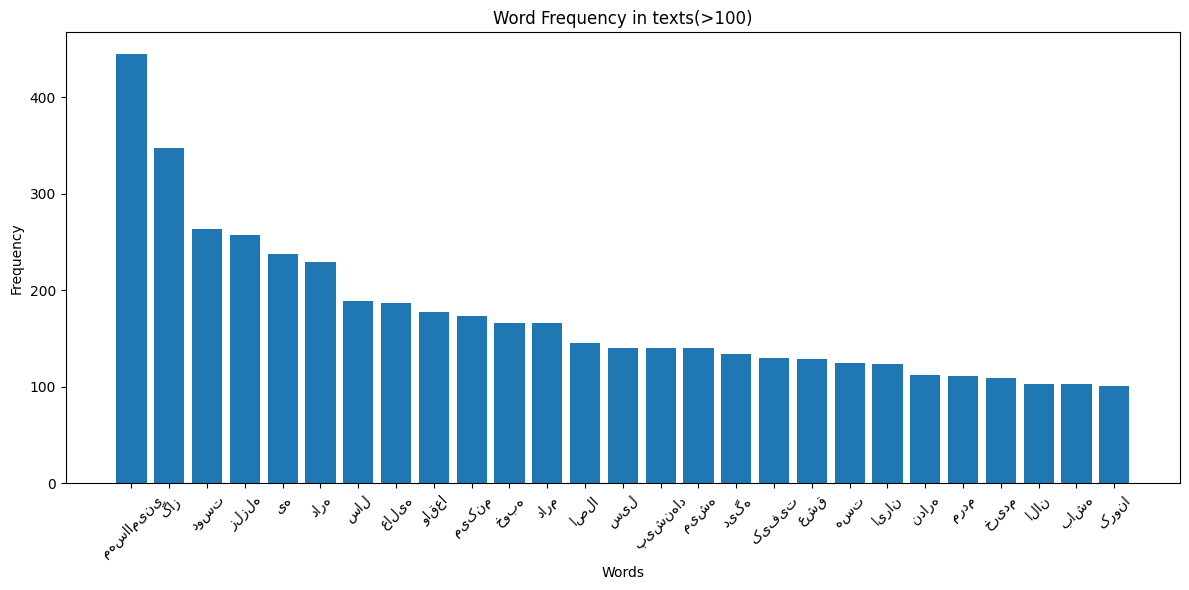
\includegraphics[width=\textwidth]{output.png}
    \caption{Word Frequency in Texts (Count > 100)}
    \label{fig:wordfreq}
\end{figure}

\section{Modeling and Classification}
We chose logistic regression as our baseline classifier due to its efficiency on sparse data (TF-IDF). The dataset was split into training and test sets, and 5-fold cross-validation was used for evaluation stability. Further, other models (e.g., decision trees, XGBoost) were explored, but initial results focused on logistic regression for clarity.

\section{Model Evaluation}
The evaluation metrics include precision, recall, F1-score, and overall accuracy.

\begin{table}[H]
\centering
\caption{Evaluation Report (Logistic Regression)}
\begin{tabular}{lcccc}
\hline
\textbf{Class} & \textbf{Precision} & \textbf{Recall} & \textbf{F1-score} & \textbf{Support} \\
\hline
ANGRY & 0.00 & 0.00 & 0.00 & 185 \\
FEAR & 0.00 & 0.00 & 0.00 & 66 \\
HAPPY & 0.31 & 0.98 & 0.47 & 306 \\
OTHER & 0.71 & 0.04 & 0.08 & 267 \\
SAD & 0.00 & 0.00 & 0.00 & 161 \\
\hline
\textbf{Accuracy} & \multicolumn{4}{c}{0.32} \\
\textbf{Macro Avg} & 0.20 & 0.21 & 0.11 & 985 \\
\textbf{Weighted Avg} & 0.29 & 0.32 & 0.17 & 985 \\
\hline
\end{tabular}
\end{table}

\section{Error Analysis}
\subsection{Class Imbalance}
The classifier is biased towards the HAPPY class due to its dominance in training samples. Other classes like FEAR and SAD are significantly underrepresented.

\subsection{Feature Limitation}
TF-IDF does not capture sequence information or context well, which might limit performance on subtle emotional distinctions.

\section{Model Monitoring and Boosting}
To enhance model performance, boosting methods like XGBoost were explored. Training and validation error curves (Figure \ref{fig:boosting}) show overfitting after several boosting rounds, emphasizing the importance of early stopping and regularization.

\begin{figure}[H]
    \centering
    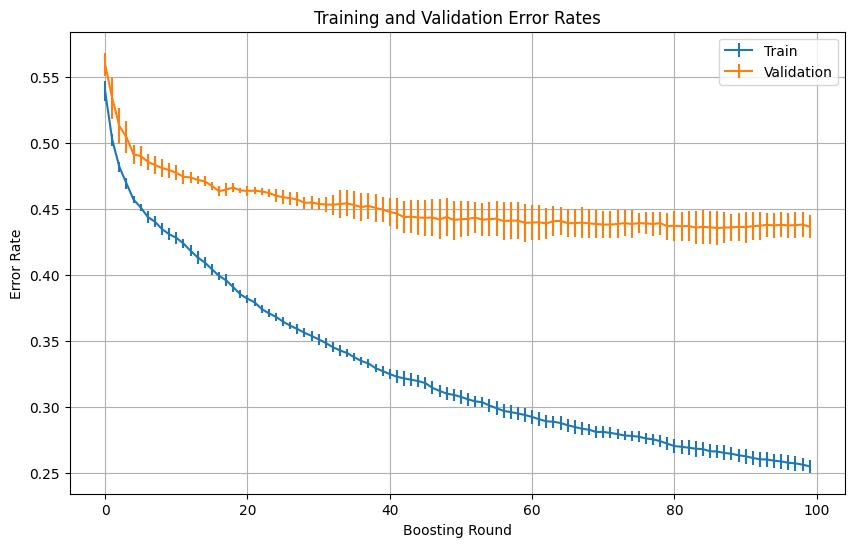
\includegraphics[width=0.8\textwidth]{output3.png}
    \caption{Training and Validation Error over Boosting Rounds}
    \label{fig:boosting}
\end{figure}

\section{Conclusion and Future Work}
This project implemented a basic yet insightful emotion detection model for Persian text using classical ML techniques. While initial results were limited by class imbalance and basic features, it laid a solid foundation. In future work, we aim to:
\begin{itemize}
    \item Use transformer-based models like BERT with fine-tuning on Persian text.
    \item Apply SMOTE or other augmentation methods for balancing classes.
    \item Explore sequence models (e.g., RNN, LSTM) with word embeddings.
\end{itemize}

\section*{Appendix}
\begin{itemize}
    \item \texttt{output.png} – Word frequency histogram
    \item \texttt{output2.png} – Class distribution chart
    \item \texttt{output3.png} – Boosting error analysis
\end{itemize}

\end{document}
